\section{Geld}
Das Geld erleichtert die Zahlungsvorgänge bei Tauschgeschäften. Als Geld können verschiedene Zahlungsmittel dienen sofern, sie folgende Ansprüchen erfüllen.
\begin{itemize}
	\item Tauschmittel reduziert Transaktionskosten des Kaufprozesses
	\item Wertaufbewahrungsmittel
	\item Masseinheit, Vergleichbarkeit des relativen Wertes von Gütern
\end{itemize}
\subsection{Wer schafft Geld}
\begin{itemize}
	\item Gold ist das anerkannte Zahlungsmittel im 15. Jahrhundert
	\item Besitzer hinterlegen Gold bei Goldschmieden. Diese stellen dafür Quittungen aus.
	\item Die Quittungen erhalten Geldcharakter (100\% Golddeckung)
	\item Goldschmiede erkennen dass über einen längeren Zeitraum nur ein Teil des hinterlegten Geldes abgeholt wird
	\item Goldschmiede beginnen überproportional viele Quittungen auszustellen
	\item Damit werden sie zu Bankiers. Keine 100\% Golddeckung sowie die Fähigkeit zur Rückzahlung basiert auf Vertrauensbasis (Zahlungsfähigkeit)
	\item Die Geschäftsbanken können heute Geld schaffen
	\item Um das Vertrauen in die Banken zu erhalten ist eine Regulierung notwendig
	\item Der Mindestreserve-Satz (RS) beschränkt Geldschöpfung
	\item Geldschöpfungsmultiplikator $GM= 1/RS$
	\item Basispunkt ist absolute Wertangabe.
	\subitem Zins von 1\% auf 2\% heisst 100 Basispunkte vergrössert
\end{itemize}
\subsection{Geldmengen}
\begin{itemize}
	\item Notenbankgeldmenge M0
	\subitem Noten und Girokonten der Geschäftsbanken
	\item Geldmenge M1
	\subitem M0 + Sichteinlagen (Zahlungszwecke)
	\item Geldmenge M2
	\subitem M1 + Spareinlagen
	\item Geldmenge M3
	\subitem M2 + Termineinlagen
	\item Die Geschäftsbanken verfügen über ein Girokonto bei der Nationalbank, dort können sie Geld mit Zinszuschlag kaufen
	\item Das erfundene Geld der Nationalbank ist Fremdkapital, weil die Girokonten den Geschäftsbanke gehören
	\item Die Geschäftsbanken können aber auch Geld bei anderen Banken zum Liborzins kaufen
\end{itemize}
\subsection{Bilanz der SNB}
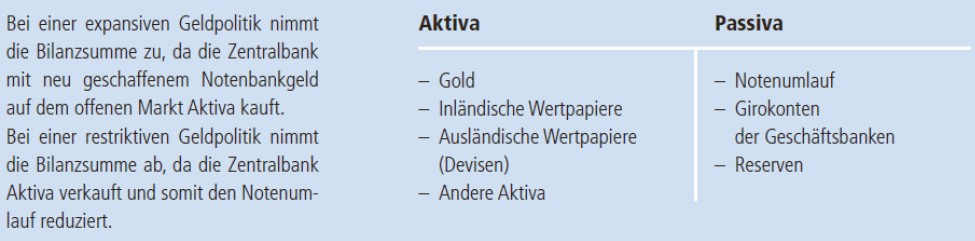
\includegraphics[width=18cm]{images/snb.jpg}
\subsection{Instrumente der Geldpolitik}
\subsubsection{Offenmarktpolitik}
\begin{itemize}
	\item Kauf und Verkauf von Wertschriften (Aktiva)
	\subitem Nationalbank bezahlt Aktiva mit frischen Geld, welches auf die Girokonten gutgeschrieben werden
	\subitem Kauf von Aktiva ist ein Repogeschäft d.h. Der Verkäufer verpflichtet sich zum späteren Rückkauf dieser Aktiva mit zusätzlichem Zins
	\item Ausgabe von Schuldverschreibungen 
\end{itemize}
\subsubsection{Mindestreservepolitik}
\begin{itemize}
	\item Nationalbank kann den Mindestreservesatz festlegen
	\item Damit wird der Geldschöpfungsmultiplikator beeinflusst
\end{itemize}
\subsection{Geldpolitische Strategien}
\begin{itemize}
	\item Wechselkursziele
	\subitem Fixierung des Wechselkurs an internationale Leitwährung
	\subitem Gefahr eines Importes von Inflation
	\item Geldmengenziele
	\subitem Monetaristischer Ansatz $P \cdot Q = M \cdot V$
	\subitem funktioniert nur solange wie V konstant ist
	\item Inflationsziele
	\subitem Wahrung der Preisstabilität
\end{itemize}
\subsection{Schweizerische Nationalbank SNB}
\begin{itemize}
	\item Vorrangiges Ziel ist die Preisstabilität und erst anschliessend die Konjunktur
	\item Der Bundesrat hat keine Weisungsbefugnis gegenüber der SNB
\end{itemize}
\vspace{1cm}